\chapter{Calibration}

\textit{Alterations of the laboratory environment combined with the exchange
of components from the original setup made it necessary to recalibrate the
setup. In this chapter we want to document the calibration steps required to
reproduce the claimed results.}

\section{Fiber coupling}

The visually shielded section of the setup, used to reduce the output power
of the laser source, is optically paired with the open section for beam
deflection via a \gls{smf} that only permits two orthogonal polarization and
a single gaussian mode. By tuning the polarisator inside the power
reduction section we can try to match one of the orthogonal polarization
modes supported by the \gls{smf}. Polarization discrepancies cause the
polarization inside the \gls{smf} to oscillate with vibrations or changes in
temperature, henceforth it is key to couple polarization modes in order to
ensure a stable operation. A strategy proven to find an approximate
polarization match between the laser beam and the \gls{smf} is presented. In
addition to the setup described in \Cref{subsec:setup_power_reduction} and
\Cref{subsec:setup_deflection_detection} an oscilloscope and a hot air gun
were used.
\begin{enumerate}
  \item Connect the photodiode to the oscilloscope and use a coarse time
    scale (i.e. \SI{2}{\second}).
  \item Apply appropriate laser safety glasses and inform present personal
    of the imminent danger.
  \item Open the cover of the power reduction setup.
  \item Apply heat to the \gls{smf} through the hot air gun, alternatively
    you can try to move the fiber.
  \item The photodiode signal should start to oscillate. Tune the polarizor
    inside the power reduction subject to minimizing the oscillation.
\end{enumerate}
The oscillations occur as the polarization circulates inside the fiber and
will stop at some point when a new equilbrium has been established. In this
case remove the heat or mechanical stress on the fiber and wait before you
reapplying new impetus.

\section{Beam alignment}

Beams that pass off-centered through spherical lenses experience optical
aberrations, additionally uncentered beams may cause further optical defects
from reflections or clipping at boundaries. Since most changes to the optical
setup outdate the previous beam alignment, hence making the realignment
a rather frequent procedure, we want to showcase what worked well for us.
As auxilliaries we used a pair of iris diaphragms that can be placed in front
of the lens mounts as a screen (i.e.\ a white sheet of hard paper). By placing
both iris diaphragms towards the incident beam on two successive lenses we
we can visually find a center reference point by inspecting the symmetry of
the iris illumination at different pinhole diameters.

\section{Camera focus}

Finally we had to reposition the camera to focus the incoming beam on the
\gls{ccd} sensor of the camera. Finding the precise focus position is not an
easy undertaking. There is no sharp focal spot but rather a focal area,
however outside the focal area no image can be seen. We followed the procedure
described in~\cite{Hertlein2017} that consists of extracting the camera rail
with its lens and focusing it on a far distant object.
\begin{figure}[htb]
  \centering
  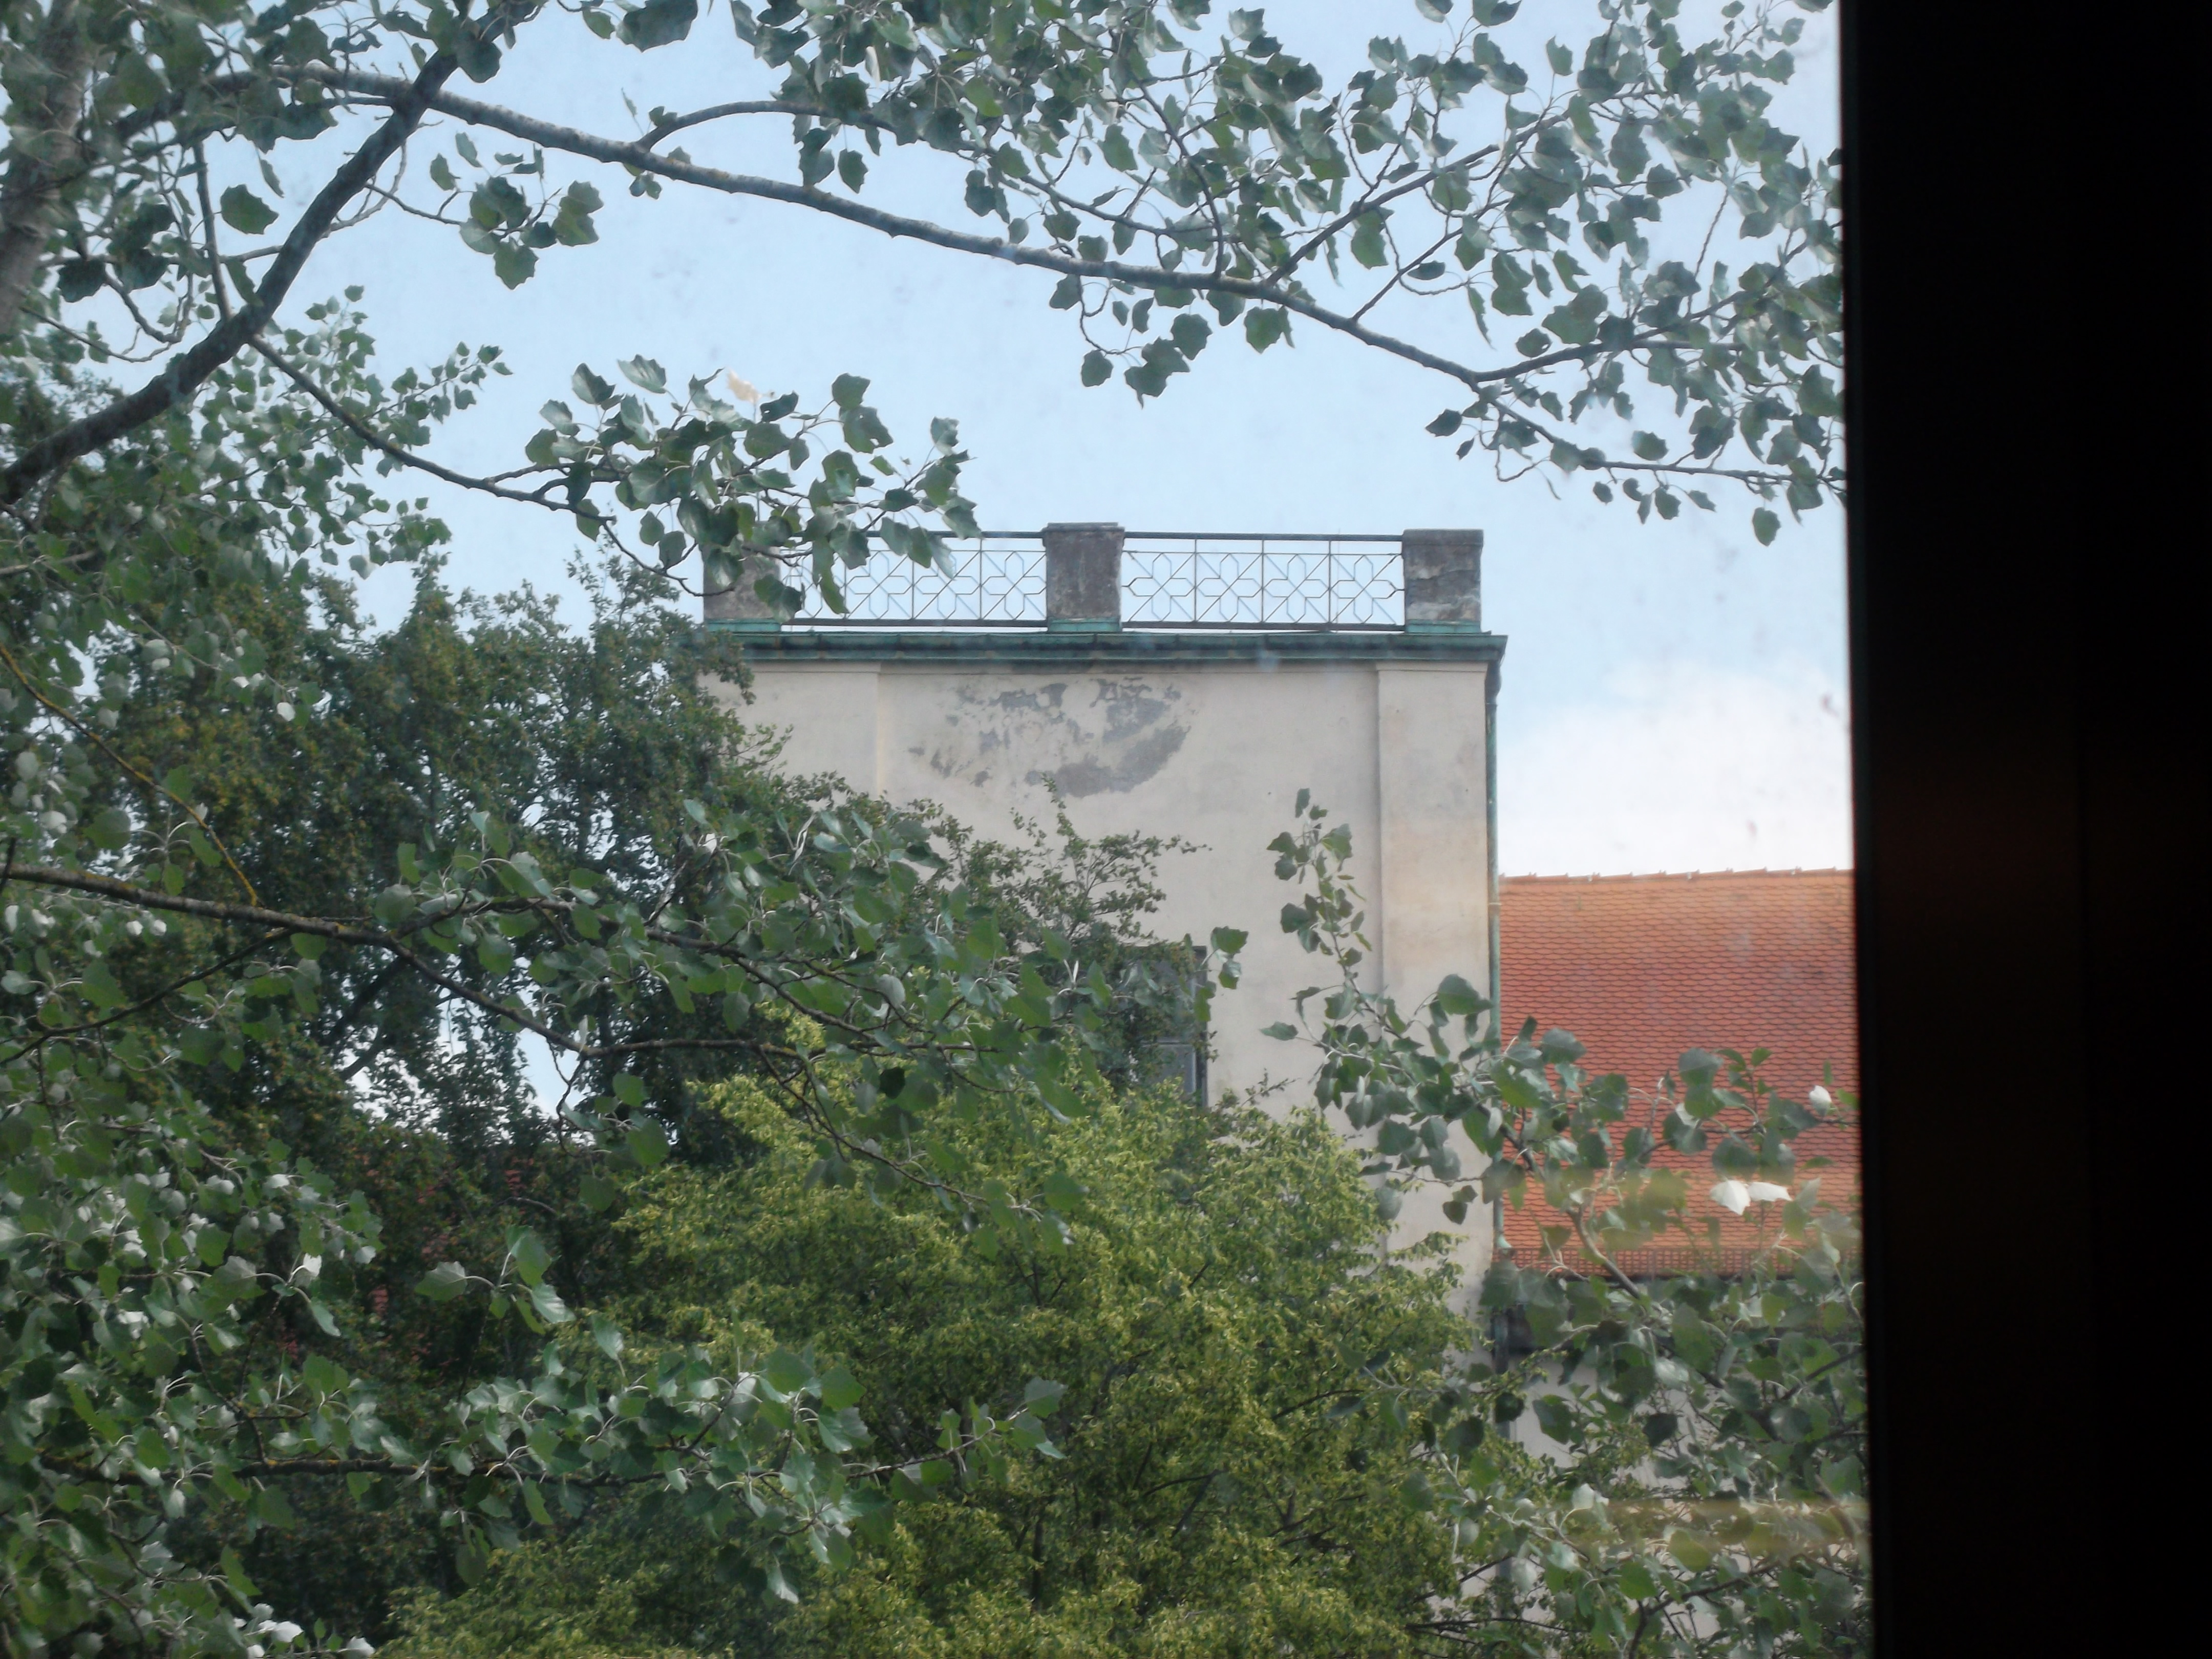
\includegraphics[width=\textwidth]{../media/image/tower.jpg}
  \caption{Focused camera with view on the balcony bars on the top of the
    university tower.
  }\label{fig:camerafocus:tower}
\end{figure}
In our case we choose the university tower as distant object. The window frame
used by~\cite{Hertlein2017} was overgrown by trees at the time of writing.
In \Cref{fig:camerafocus:tower} we can see the university tower as seen by
a common digital camera. If we look careful on the left-hand side of the
tower top we discover a weathercock.
\begin{figure}[htb]
  \centering
  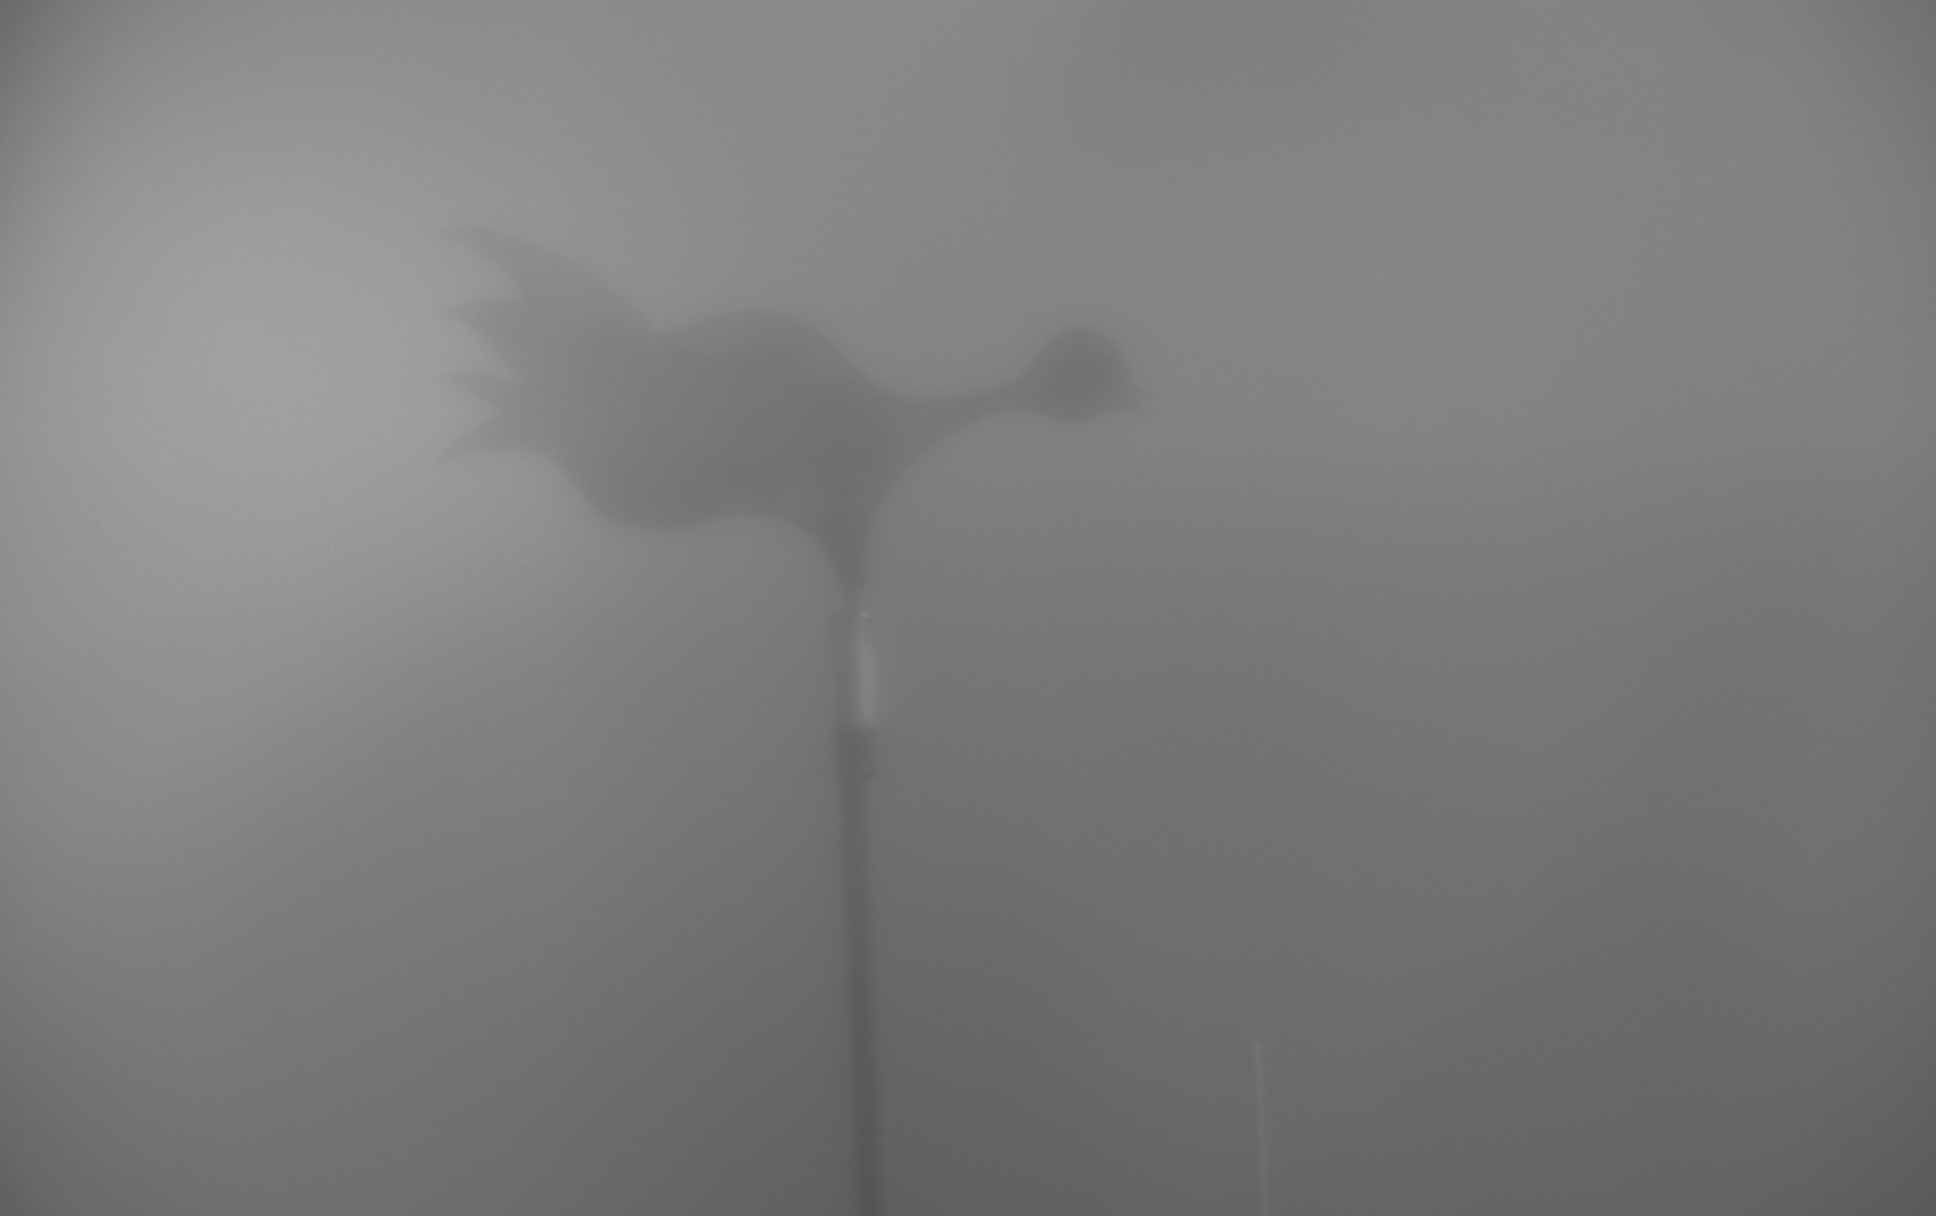
\includegraphics[width=\textwidth]{../media/image/focus.jpg}
  \caption{Focused camera with view on the weather cock on the top of the
    university tower.
  }\label{fig:camerafocus:focus}
\end{figure}
In \Cref{fig:camerafocus:focus} we can see the weathercock on top of the
university tower as seen by the \gls{ccd} camera at aligned focal position.
